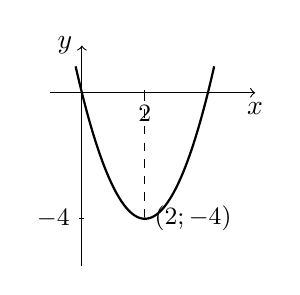
\begin{tikzpicture}[scale=0.4]
    \draw[->] (-1,0) -- (5.5,0) node[below] {$x$};
    \draw[->] (0,-5.5) -- (0,1.5) node[left] {$y$};

    \draw (2,0.08) -- (2,-0.08) node[below] {\small $2$};
    \draw (0,-4) ++(0.08,0) -- ++(-0.16,0) node[left] {\small $-4$};

    \draw[dashed] (2,0) -- (2,-4);
    \draw[thick, domain=-0.2:4.2, samples=200] plot (\x,{(\x-2)^2-4});

    \fill (2,-4) circle (1.3pt);
    \node[right] at (2,-4) {\small $(2;-4)$};
\end{tikzpicture}
